\chapter{Experiments: Regular Tilings}

% (TODO): Overall: standard deviations.

% (TODO): Remember to always specify specifics of experiment setups for all
% experiments

\textcolor{red}{
  \textbf{Methodology:} We look at the three most common types of tilings by
regular polygons: regular tilings. Grünbaum and Shephard (section 1.3) about
tilings, talks about regularity. ``Edge-to-edge'' tiling by congruent regular
polygons. The three regular tesselations, or Euclidean tilings, are square,
triangular, and hexagonal.
}

\textcolor{red}{
  There also exists semiregular, often called uniform, tilings, where there are
two or more faces. There are also more complex schemes, but we are interested in
tilings that are lattice-like. The different types of Bravais lattices for 2
dimensions were all investigated, but using just regular tilings was found to be
sufficient. We are not necessarily interesting in comparing lattice structures
directly, but rather in the applicability of such structures in general.
}

\textcolor{blue}{
  ``Lattice networks/models are common in computational physics, condensed
matter physics and beyond, modelling physical interactions, phase transitions
and structure [15]. Examples include: discrete lattices like the Ising model
with variables representing magnetic dipole moments of atomic spins, and the
Gray- Scott reaction-diffusion model to simulate chemical systems [22]. Also,
physical substrates often have a regular grid of connections. Lattice networks
are therefore more realistic representations of many physical systems that would
be considered for reservoir computing.'', Role of Structure and Complexity, Dale
et al.
}

% (TODO): t!
\begin{figure*}[t]
  \centering
  \begin{subfigure}{.32\textwidth}
    \centering
    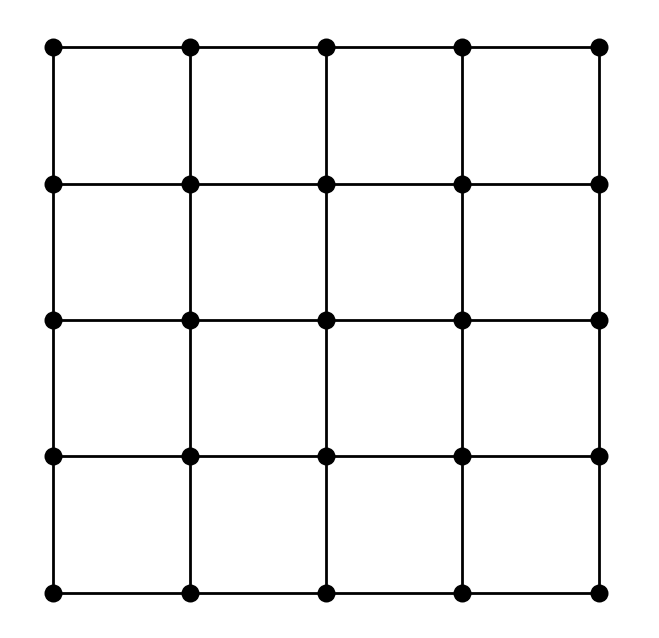
\includegraphics[width=1.0\linewidth]{figures/square.png}
    \label{fig:rt-square}
  \end{subfigure}
  \begin{subfigure}{.32\textwidth}
    \centering
    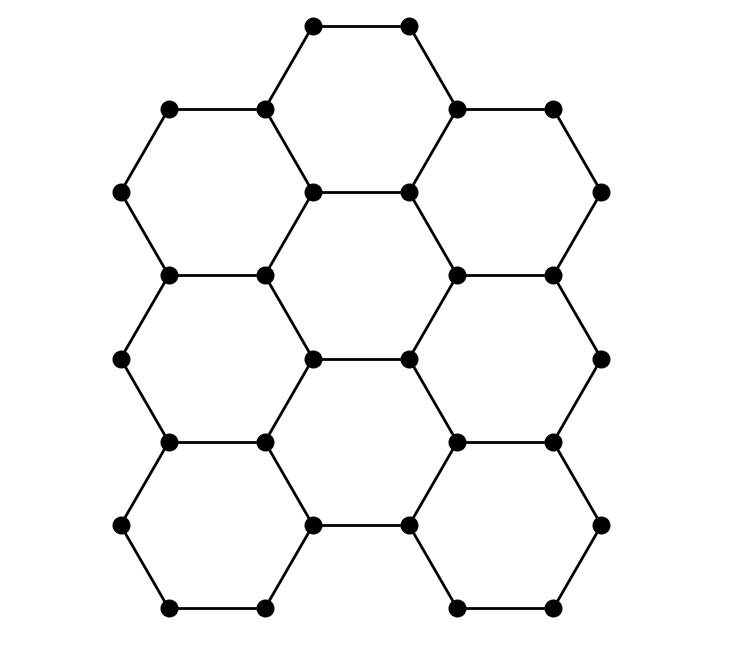
\includegraphics[width=1.0\linewidth]{figures/hex.png}
    \label{fig:rt-hex}
  \end{subfigure}
  \begin{subfigure}{.32\textwidth}
    \centering
    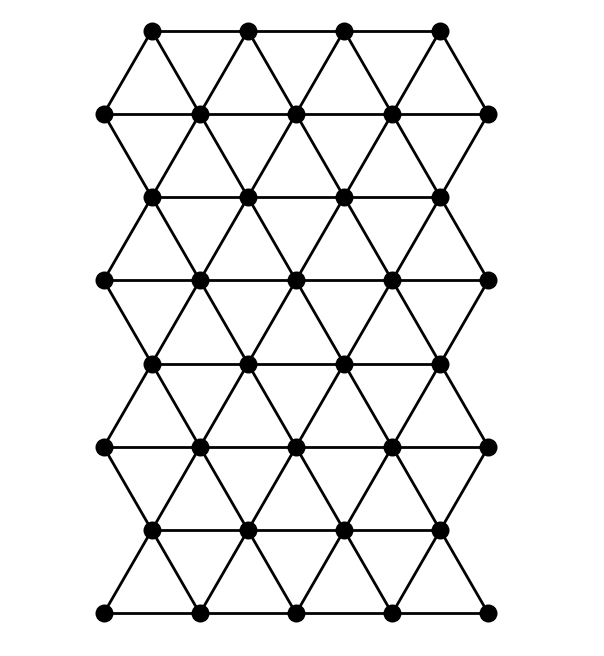
\includegraphics[width=1.0\linewidth]{figures/triangular.png}
    \label{fig:rt-tri}
  \end{subfigure}
  \caption{
    Regular tilings investigated for their quality as reservoir
topologies. Investigated topologies include square (a), hexagonal (b), and
triangular (c) regular tilings.
  }
  \label{fig:regular-tilings}
\end{figure*}

\section{Methodology}

% (TODO): Chapter reference.
\textcolor{red}{
  \textbf{Methodology:} We use the same base as provided by the chapter on
methodology, but replace the weight matrix of the reservoir, i.e. its innards,
with that of the lattice structures we generate. This provides connectivity
within the reservoir of regular, spatially constrained nature. Everything else
should be the same.
}

\section{Reservoir Quality of Regular Tilings}

\subsection{Synopsis}

\subsection{Results and Discussion}

% (TODO): t!
\begin{figure}[h!]
  \centering
  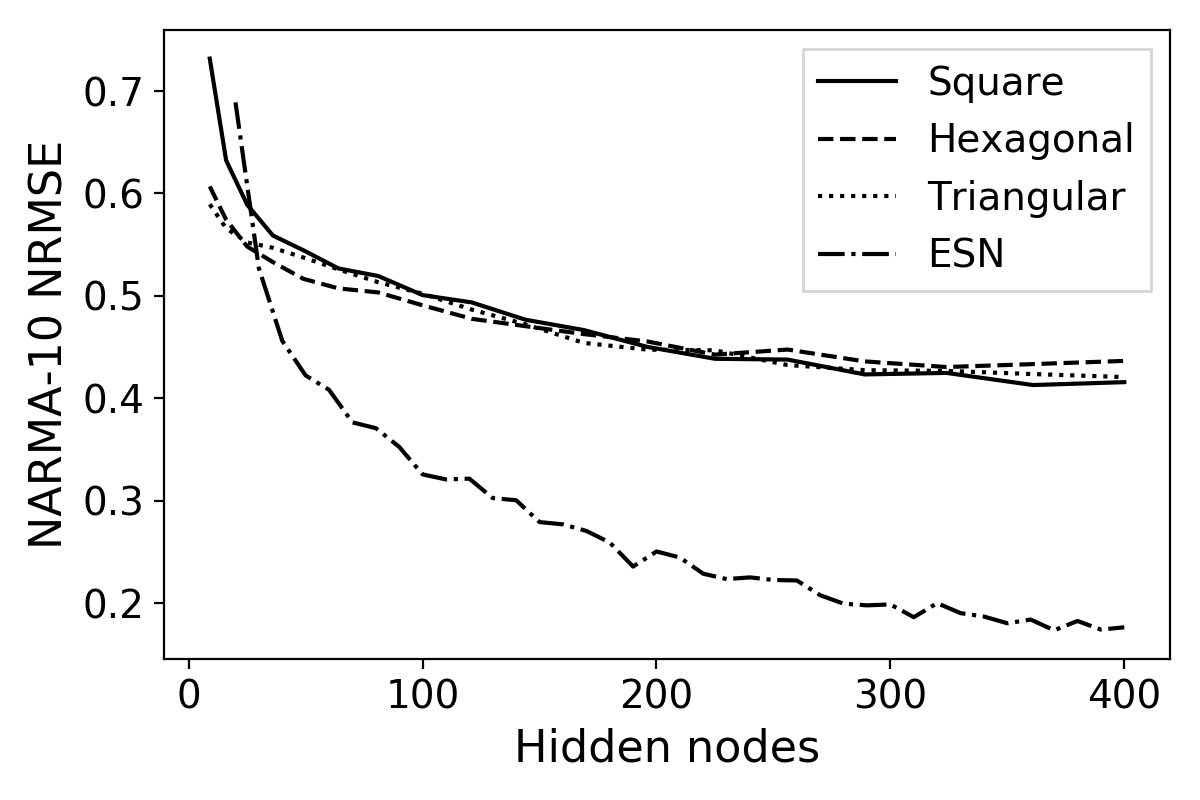
\includegraphics[width=3.5in]{figures/regular-tilings-performance.png}
  \caption{
    Performance of square, hexagonal, and triangular regular tilings as
reservoir topologies without other modifications to the echo state network
methodology.
  }
  \label{fig:rt-performance}
\end{figure}

\textcolor{red}{
  Again, we see that restricting topologies with no other changes will result in
a performance penalty, seen in Figure \ref{fig:rt-performance}.
}

% (TODO): t!
\begin{figure*}[t]
  \centering
  \begin{subfigure}{.32\textwidth}
    \centering
    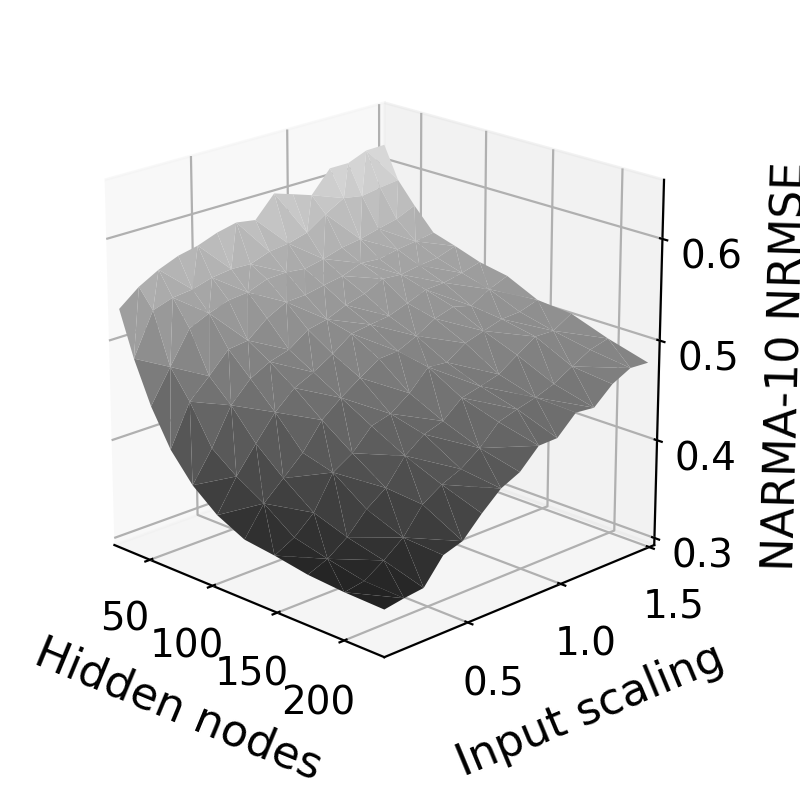
\includegraphics[width=1.0\linewidth]{figures/regular-tilings-performance-is-sq.png}
    \caption{}
    \label{fig:rt-is-square}
  \end{subfigure}
  \begin{subfigure}{.32\textwidth}
    \centering
    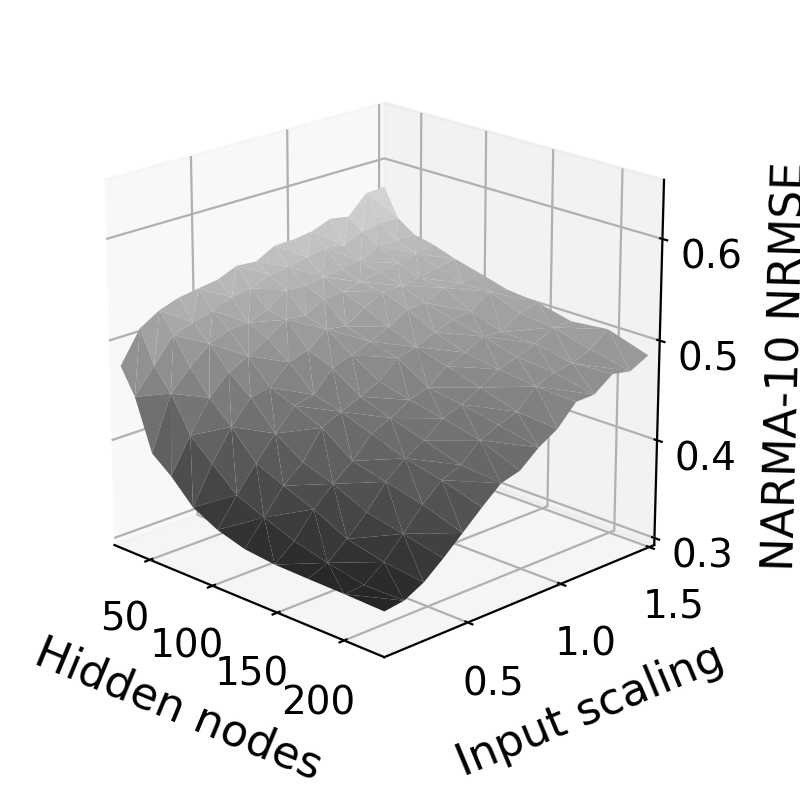
\includegraphics[width=1.0\linewidth]{figures/regular-tilings-performance-is-hex.png}
    \caption{}
    \label{fig:rt-is-hex}
  \end{subfigure}
  \begin{subfigure}{.32\textwidth}
    \centering
    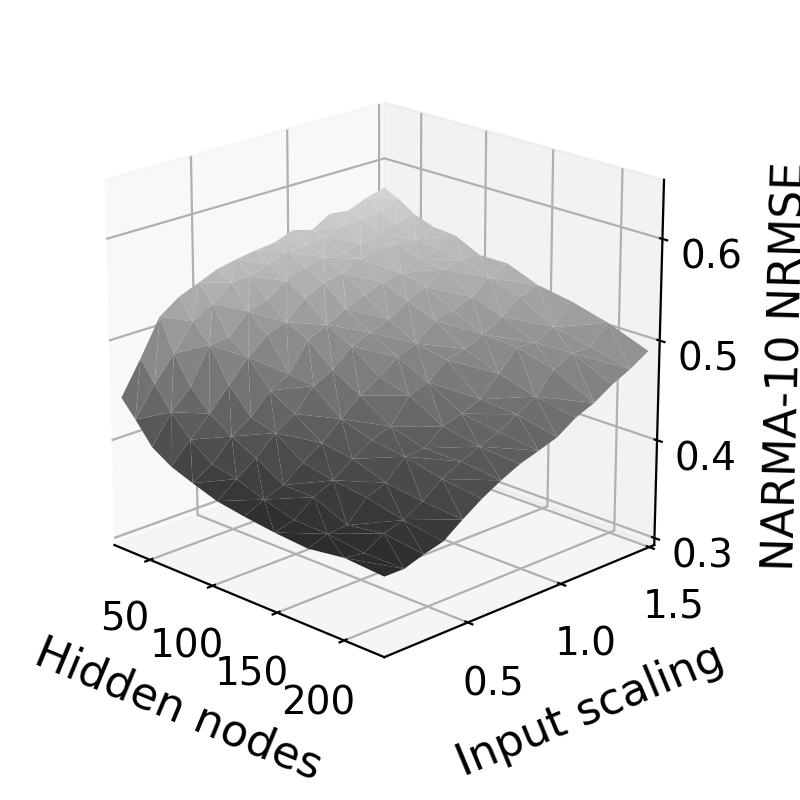
\includegraphics[width=1.0\linewidth]{figures/regular-tilings-performance-is-tri.png}
    \caption{}
    \label{fi:rt-is-tri}
  \end{subfigure}
  \caption{
    Regular tilings investigated for their quality as reservoir topologies, here
as a function of reservoir size and input scaling. Investigated topologies
include square (a), hexagonal (b), and triangular (c) regular tilings.
  }
  \label{fig:rt-performance-is}
\end{figure*}

% (TODO): ref.
\textcolor{red}{
  Further, we investigate the impact of input scaling using what we found in
Chapter ?, as input plays a critical role in input retention. Here, the question
is perhaps not ``exactly how good can we make the topologies with input
scaling'', but we are instead interested in the fact that it does matter at all,
as we can use this in further experiments. We see in Figure
\ref{fig:rt-performance-is} that lowering the input scaling again improves
performance significantly, perhaps again due to issues with memory capacities.
}

\subsection{Summary}

\section{Regular Tilings with Directed Edges}

\subsection{Synopsis}

% (TODO): ref.
\textcolor{red}{
Using knowledge obtained in Chapter ?, we modify the resulting networks to have
directed edges, and scale the input magnitude to find a suitable one.
}

\subsection{Results and Discussion}

% (TODO): t!
\begin{figure*}[t]
  \centering
  \begin{subfigure}{.40\textwidth}
    \centering
    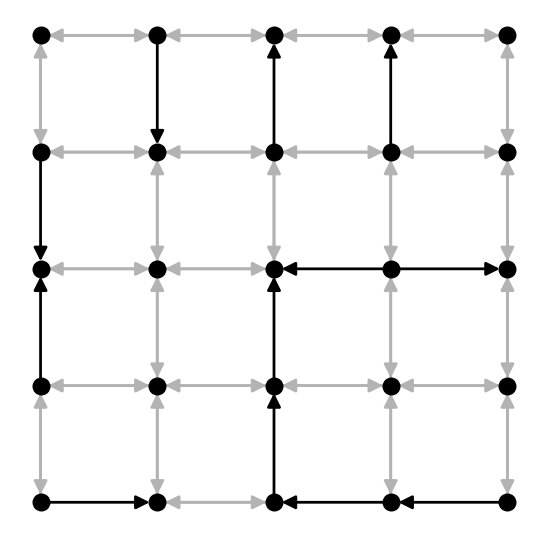
\includegraphics[width=1.0\linewidth]{figures/dir_lattice_025.png}
    \caption{}
    \label{fig:dir-lattice-a}
  \end{subfigure}
  \hspace{25pt}
  \begin{subfigure}{.40\textwidth}
    \centering
    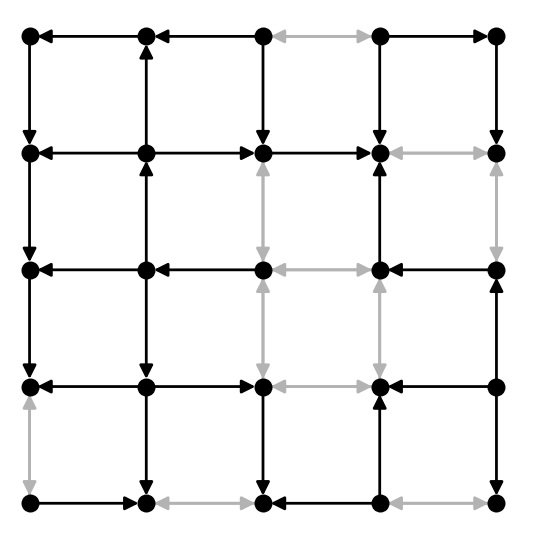
\includegraphics[width=1.0\linewidth]{figures/dir_lattice_075.png}
    \caption{}
    \label{fig:dir-lattice-b}
  \end{subfigure}
  \caption{
    Example square grids where 25\% (a) and 75\% (b) of the undirected edges are
made directed instead.
  }
  \label{fig:dir-lattice}
\end{figure*}

% (TODO): t!
\begin{figure*}[t]
  \centering
  \begin{subfigure}{.32\textwidth}
    \centering
    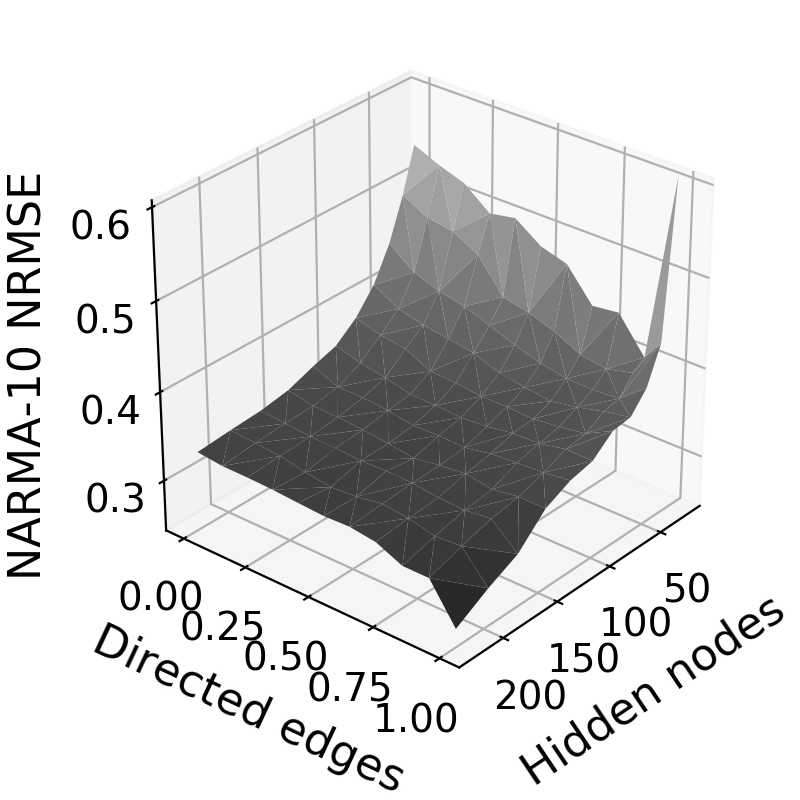
\includegraphics[width=1.0\linewidth]{figures/rt-dir-perf-sq.png}
    \caption{}
    \label{fig:rt-dir-perf-trisurf-sq}
  \end{subfigure}
  \begin{subfigure}{.32\textwidth}
    \centering
    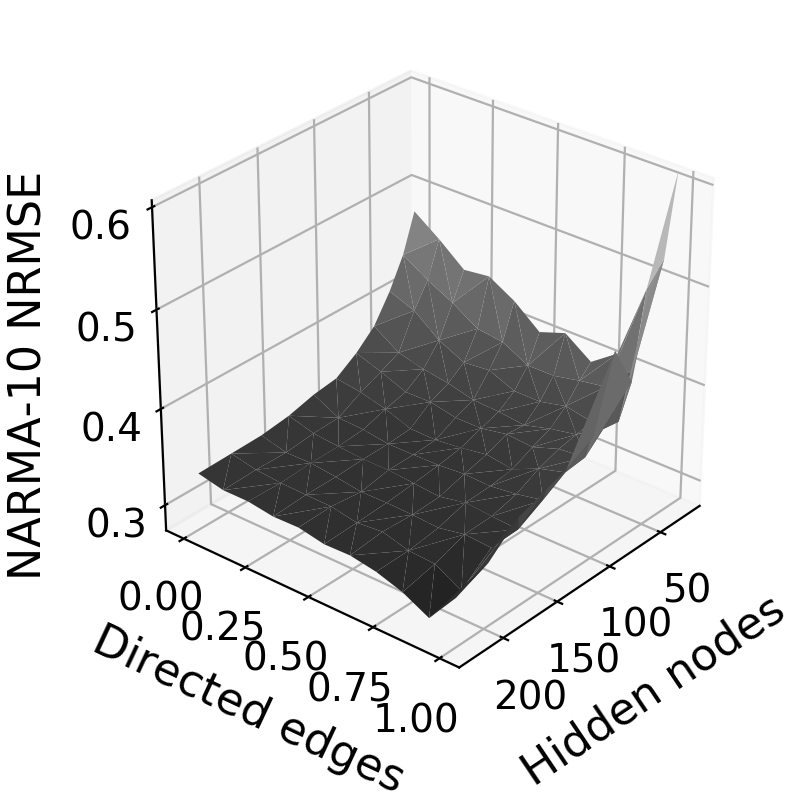
\includegraphics[width=1.0\linewidth]{figures/rt-dir-perf-hex.png}
    \caption{}
    \label{fig:rt-dir-perf-trisurf-hex}
  \end{subfigure}
  \begin{subfigure}{.32\textwidth}
    \centering
    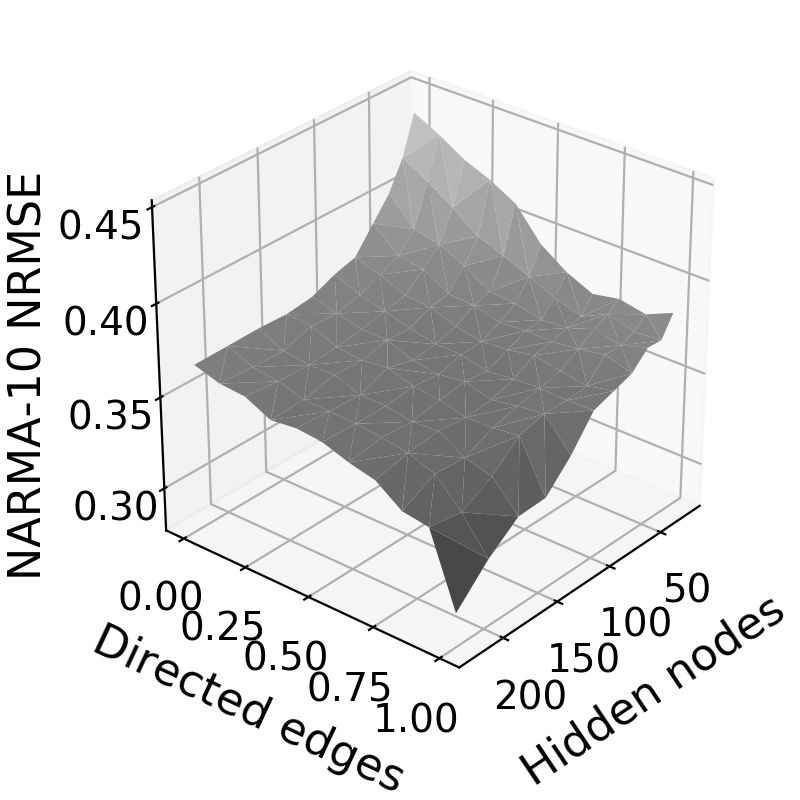
\includegraphics[width=1.0\linewidth]{figures/rt-dir-perf-tri.png}
    \caption{}
    \label{fig:rt-dir-perf-trisurf-tri}
  \end{subfigure}
  \caption{
    \textcolor{red}{No caption yet.}
  }
  \label{fig:rt-dir-perf-trisurf}

  \centering
  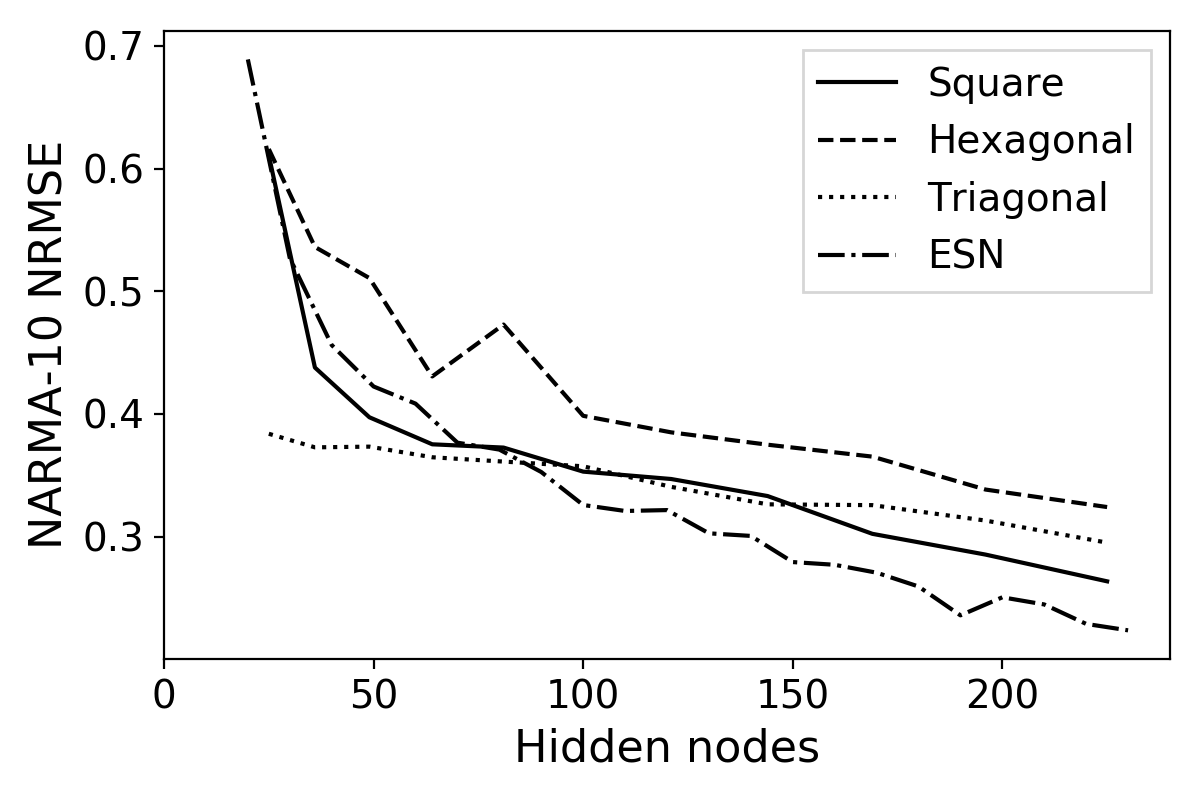
\includegraphics[width=3.5in]{figures/rt-dir-perf.png}
  \caption{\textcolor{red}{No caption yet here.}}
  \label{fig:rt-dir-perf}
\end{figure*}

\textcolor{red}{
  We see that directed edges make the grids perform quite close to ESNs on the
NARMA-10 dataset. We choose the square lattice to move further, as they are all
quite similar, but the square one seems most stable and performs very well.
}

\begin{figure}
  \centering
  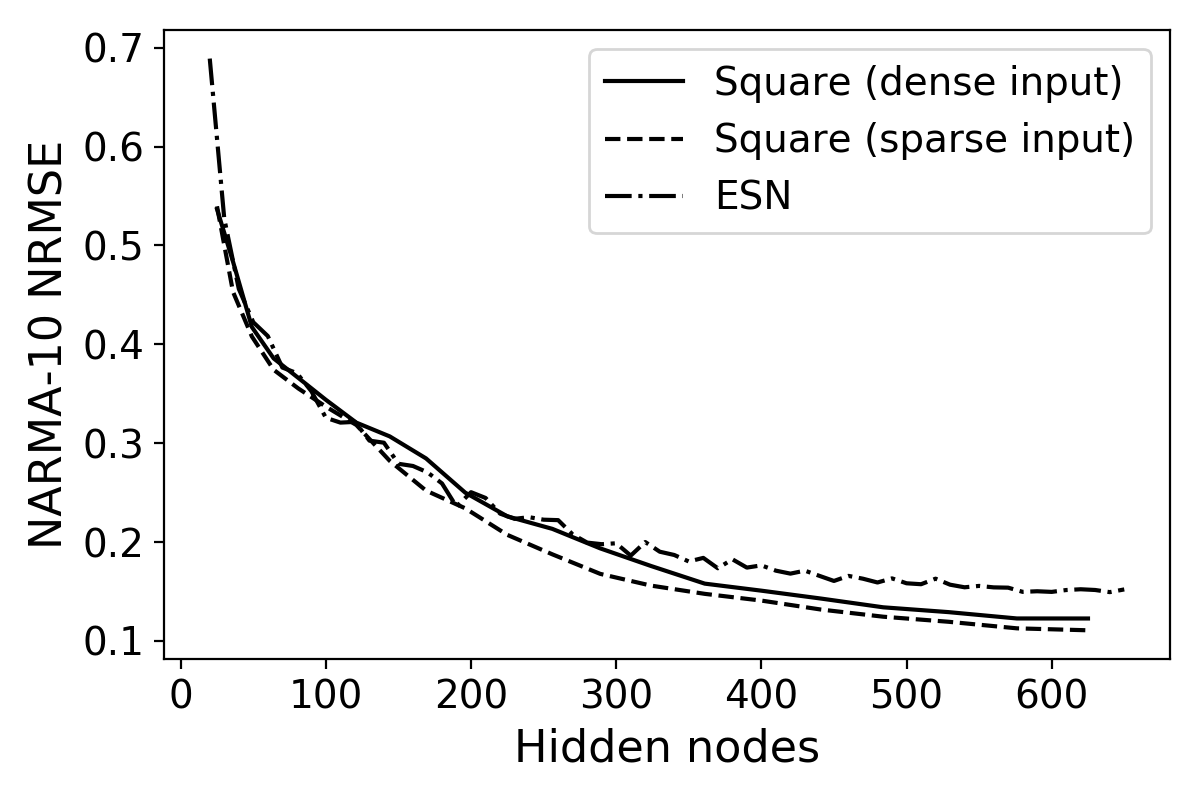
\includegraphics[width=3.5in]{figures/rt-performance-big.png}
  \caption{\textcolor{red}{No caption here yet.}}
  \label{fig:rt-performance-big}
\end{figure}

\textcolor{red}{
  When we introduce a global input scheme, the square grids get even
better. This is crazy. The square grids do not plateau nearly as much as the
ESNs. In fact they get much better. We also add sparse input matrices, which
means only 50\% of the hidden nodes see the input.
}

% (TODO): t!
\begin{table}[t]
  \centering
  \begin{center}
    \caption{\textcolor{red}{No caption here yet.}}
    \label{tab:sq-global-input}
    \begin{tabular}{c c c c c}
      \hline
      \thead{Reservoir type} & \thead{Hidden \\ nodes} & \thead{Unique \\ input weights} & \thead{Unique \\ reservoir weights} & \thead{NARMA-10 \\ NRMSE} \\
      \hline
      \rule{0pt}{2.5ex} Square grid & 100 & 1 & 1 & 0.0 \\
      ESN & 100 & 1 & 1 & 0.0 \\
      Square grid & 225 & 1 & 1 & 0.0 \\
      ESN & 225 & 1 & 1 & 0.0 \\
      Square grid & 400 & 1 & 1 & 0.0 \\
      ESN & 400 & 1 & 1 & 0.0\rule[-1ex]{0pt}{0pt} \\
      \hline
    \end{tabular}
  \end{center}
\end{table}

\textcolor{red}{
  Think about including activations of hidden nodes, as it is so clear that they
all see the same input.
}

\textcolor{red}{
  Should we also include an image of actual prediction, to show how good it is?
}

\textcolor{red}{
  We should maybe also compare MC and KQ/G to that of ESNs, as independent
metrics.
}

\textcolor{red}{
  Should we include experiments with harder NARMA? I think there is already
quite a lot of information, so this might not really be necessary.
}

\subsection{Summary}

\section{Shrinking and Growing Directed Reservoirs}

\subsection{Synopsis}

\subsection{Results and Discussion}

Should include both shrinking and growing reservoirs for a conjoined discussion.

\subsection{Summary}

\section{Restoring Bidirectional Edges}

\subsection{Synopsis}

\subsection{Results and Discussion}

\subsection{Summary}

\section{Conclusion}


%%% Local Variables:
%%% mode: latex
%%% TeX-master: "../thesis"
%%% End:
